% Introduction
\section{Introduction}

%%%%%%

% Cite:
% Wireless sensor networks	#yick2008wireless
% Mobile campus networks 	#hernandez2005comparative
% Mobile gaming community	#cunningham2002optimizing
% Energy-efficient network	#jones2001survey
% Internet of things 			#qin2014software
% Connectivity  			#moscibroda2006complexity
% Density					#wang2015connectivity

% The cite of the existing algorithms are listed in related work

%%%%%%

% Paper Logical Flow
% P1-P2 Background
% P3-P6 motivation
% P7-P11 contribution
% P12 structure

% P1:    
% Define realistic network
% General background
% The situation&scenario our research applies to
The growing interest in the Internet of Things (IoT) has resulted 
in a number of wide-area deployments of wireless networks \cite{qin2014software},
such as wireless sensor networks \cite{yick2008wireless}, mobile campus networks 
\cite{hernandez2005comparative}, mobile gaming community \cite{cunningham2002optimizing}, etc.
All these realistic networks possess multi-hop and large-scale characteristics obviously.

% P2: 
% Why NB problem is related and important to the background in P1  
% Define what is neighbor and what is neighbor discovery problem
% A brief introduction of the existing works and explain deterministic and probabilistic with one sentence each
Neighbor discovery is a fundamental step of constructing a wireless network, based on 
which the network can implement further applications such as routing and broadcasting.
The core target is for each node in the network to discover the nodes in its radio sensing range 
with one-hop communication, which are called neighbors. 
A number of existing methods \cite{dutta2008practical, kandhalu2010u,
bakht2012searchlight, sun2014hello, chen2015heterogeneous,
wang2015blinddate, qiu2016talk, mcglynn2001birthday,
vasudevan2009neighbor, you2011aloha, song2014probabilistic} have been proposed 
to deal with this issue, some of which are based on deterministic techniques, 
those turn on the radio with deterministic sequences,
while others are probabilistic approaches, those turn on the radio with different probabilities.


% P3:
% Crucial problem:  collision issue in a partially-connected network
% What is a practical network model and define what is a partially-connected network
Unfortunately, despite great efforts, neighbor discovery in a realistic network remains an open problem.
The key issue lies in the collision condition in the large-scale networks.
In a large-scale network, each node is only able to sense the 
nodes if their Euclidean distance is no more than a given threshold 
based on received signal strength \cite{moscibroda2006complexity, wang2013gaussian, wang2015connectivity}.  
We call this multi-hop wireless networks connectivity as \emph{partially-connected}.


% P4: 
% What issues will occur, if transferring the deterministic methods to the partially-connected network
% On the one hand,
As for the deterministic approaches, they only deal with the neighbor discovery problem for two nodes.
When transferred to multiple nodes scenario, they can not solve the collision issue when more 
than one neighbors are transmitting simultaneously. 


% P5:
% What issues will occur, if transferring the probabilistic methods to the partially-connected network
% On the other hand,
Relatively, probabilistic approaches can deal with multiple nodes discovery well but only consider
the network is fully-connected, the topology of which is a complete graph. 
Therefore in the large-scale network where the nodes are partially-connected,  
the probability adopted in these approaches can not be desirable 
and thus can not reduce the collision efficiently. 
To our best knowledge, no relevant researches 
have focused on the neighbor discovery problem in the large-scale networks 
where nodes are partially-connected.


% P6: 
% Summarize our initiative insight
Our initiative insight is to take the distribution of the nodes in the network
into fully consideration, since in a wireless network the distribution of 
nodes' deployment directly plays a vital role in determining the intrusion 
detection capability of a communication device.

% P7:
% Our solution/contribution : we propose Alano algorithm based on the distribution of nodes for the partially-connected networks
In this paper, we propose Alano\footnote{Alano is the god of luck in Greek mythology.}, 
a nearly optimal probability based algorithm to discover neighbors in partially-connected networks. 
As fully studied in \cite{wang2013gaussian} , the nodes in wireless sensor networks are likely to 
follow a uniform or a Gaussian distribution as showed in Fig. \ref{distribution}, 
depending on the specific network applications, which is taken into consideration of the proposed Alano algorithm.

 
 \begin{figure}[!t]
\centering
\subfigure[uniform distribution]{\includegraphics[width=1.7in]{./Figure/uniform.eps}}
\vspace{0.03in}
\subfigure[Gaussian distribution]{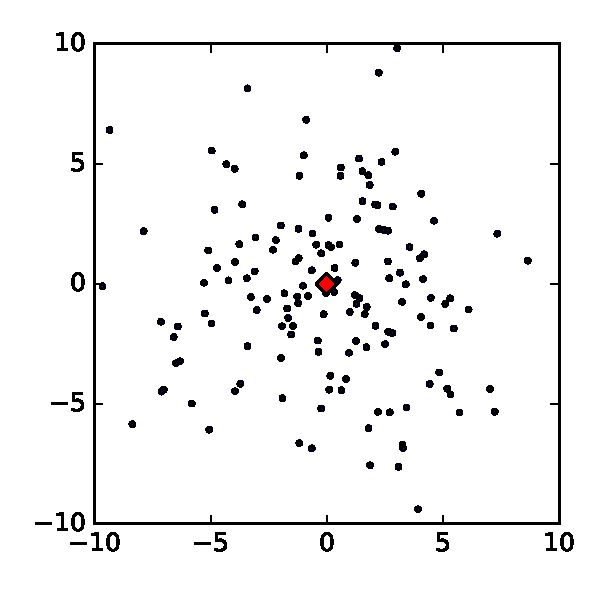
\includegraphics[width=1.7in]{./Figure/normal.eps}}
\caption{WSN deployments following uniform and Gaussian distribution.}
\label{distribution}
%\vspace{-0.2in}
\end{figure}


% P8: 
% A special type of partially-connected networks: energy-efficient network
In addition, among the large-scale networks, there is a special 
type named energy-efficient network \cite{jones2001survey}.
Wireless sensor network is a typical energy-efficient network that all the sensor nodes have to maintain 
strict power budgets to attain years of lifetime\cite{dunkels2011contikimac}.
Duty cycle mechanism, the fraction of time the radio is turned on, is 
utilized to raise the power-awareness of the nodes in the network.
Correspondingly, the neighbor discovery process 
needs adjustments to deal with the dilemma between 
a balance of energy-efficiency and low-latency.


% P9: 
% For energy-efficient networks, we propose RDS-Alano in global duty cycle scenario 
% and TP-Alano in the local duty cycle scenario.
For energy-efficient networks, we design deterministic methods
to align the wake-up time slots between the neighbors to achieve lower latency bound.
Specifically, We propose RDS-Alano algorithm for the symmetric energy-efficient networks, where 
all the nodes share a identical duty cycle $\theta$ and TP-Alano for the
asymmetric energy-efficient networks where each node possesses a respective duty cycle $\theta_i$. 


% P10:
% Simulation results support our high performance
Our simulation under the practical distribution of networks 
\cite{wang2013gaussian} shows the proposed Alano algorithm
holds significant strengths than the state-of-the-art methods,
based on the evaluation of speed, quality and scalability.% and robustness 
Alano achieves 31.35\% to 32.32 times lower latency
and has higher discovery rate during the whole process of neighbor discovery, 
no matter in symmetric or asymmetric scenario and in uniform or Gaussian distribution.
When the number of nodes increases and the network becomes denser, 
Alano still keeps its high performance. 


% P11:
% Contribution summarize
The main contributions of this paper are summarized as follows:
\begin{itemize}
\item[1)] We model the distribution of node deployment with mathematical analysis 
and analyse the expectation number of neighbors of a node in uniform distribution and Gaussian
distribution.
\item[2)] We propose Alano, a low-latency strategy to achieve neighbor discovery process
in a large-scale network.
\item[3)] We propose a Relaxed Difference Set based Alano algorithm (RDS-Alano) 
to achieve low-latency neighbor discovery process in the symmetric energy-efficient networks. 
\item[4)] We propose a Traversing Pointer based Alano algorithm (TP-Alano) to
achieve low-latency neighbor discovery process in the asymmetric energy-efficient networks. 
\end{itemize}


% P12:
% Remaining structure
The remainder of the paper is organized as follows.
The next section highlights some related work and 
puts forward some serious problems. 
Some notion definitions and the system model are given in Section \ref{sectionmodel}. 
We analyse the node's expectation number of neighbors and 
propose Alano algorithm in \ref{PCN} as a foundation.
Section \ref{EEN} describes the RDS-Alano algorithm for 
symmetric scenario and TP-Alano algorithm for asymmetric scenario
respectively in energy-efficient networks.
We have conducted extensive simulations, and the results are shown in Section
\ref{Evaluation}. Finally, we conclude the paper in Section
\ref{Conclusion}.

